% A fictional two-column paper used to demo paper-annotate. Nothing in it is real.
\documentclass[10pt,twocolumn,letterpaper]{article}
\usepackage[margin=0.85in,columnsep=0.3in]{geometry}
\usepackage{times}
\usepackage{amsmath,amssymb}
\usepackage{booktabs}
\usepackage{tikz}
\usepackage[hidelinks]{hyperref}

\title{\textbf{Tidewater: Forecasting Dock Demand for City Bike Rebalancing}}
\author{Demo Author\\{\small A fictional paper for trying out paper-annotate}}
\date{}

\begin{document}
\maketitle

\begin{abstract}
Bike-sharing systems lose riders when docks are empty in the morning and full in the evening.
Operators rebalance the fleet with trucks, but routes are planned from yesterday's counts and react late to weather and events.
We present Tidewater, a lightweight forecaster that predicts hourly dock demand from trip histories, weather, and a calendar of local events.
Tidewater couples a shared temporal encoder with a small per-station head, so a new station can be added with a few days of data.
On three simulated city networks, Tidewater reduces empty-dock hours by 18\% relative to a seasonal baseline while planning shorter truck routes.
\end{abstract}

\section{Introduction}

A shared bike is only useful if a dock is available at both ends of the trip.
In most cities, commuting flows move bikes from residential areas to business districts in the morning and back in the evening.
Without intervention, the outer stations empty out and the central ones overflow within a few hours.

Operators respond by moving bikes with trucks overnight and during the day.
These rebalancing routes are usually planned from the previous day's counts, which works on ordinary weekdays but fails on rainy mornings, public holidays, and evenings with large concerts.
A forecaster that anticipates such deviations would let operators move bikes before the shortage appears.

Existing approaches either fit one model per station, which needs months of history, or a single global model, which blurs the differences between a suburban rail stop and a downtown plaza.
Tidewater sits between the two.
A shared encoder learns how weather and events shift demand across the whole city, and a small head per station learns its local rhythm.
Our contributions are a forecasting architecture that adapts to new stations with little data, an evaluation protocol based on empty-dock hours rather than prediction error alone, and a study of how forecast quality translates into truck route length.

\section{Method}

\paragraph{Problem setup.}
Let $x_{s,t}$ be the number of bikes taken from station $s$ during hour $t$, and let $c_t$ collect the weather and calendar features for that hour.
Given the last $H$ hours, we predict demand for the next $F$ hours at every station.

\paragraph{Shared encoder.}
The encoder maps the recent history of all stations and the context features to a city-level state,
\begin{equation}
  h_t = \mathrm{GRU}\big(h_{t-1},\, [\bar{x}_{t};\, c_t]\big),
  \label{eq:encoder}
\end{equation}
where $\bar{x}_t$ is the vector of normalized station counts.
Because the state is shared, a rainy morning observed at one station informs the forecast at all others.

\paragraph{Station heads.}
Each station $s$ owns a two-layer head $g_s$ that turns the city state into a local forecast, $\hat{x}_{s,t+1:t+F} = g_s(h_t)$.
New stations start from the average of their nearest neighbours' heads and are fine-tuned once a few days of trips are available.

\paragraph{Training objective.}
We minimize a Poisson negative log-likelihood, which suits count data and penalizes underestimating busy hours more than a squared error would.

\section{Experiments}

\paragraph{Setup.}
We simulate three networks of 120, 260, and 410 stations with commuting, leisure, and event-driven trips.
Each network has one year of training data and two months of test data.
We compare against a seasonal baseline that repeats last week's demand, a per-station gradient-boosted model, and a single global recurrent model.

\begin{table}[t]
  \centering
  \small
  \begin{tabular}{lccc}
    \toprule
    Method & MAE $\downarrow$ & Empty h $\downarrow$ & Route km $\downarrow$ \\
    \midrule
    Seasonal       & 2.41 & 1{,}930 & 412 \\
    Per-station    & 2.05 & 1{,}744 & 398 \\
    Global GRU     & 1.97 & 1{,}702 & 391 \\
    Tidewater      & \textbf{1.82} & \textbf{1{,}583} & \textbf{377} \\
    \bottomrule
  \end{tabular}
  \caption{Results on the 260-station network. Empty h counts station-hours with no bike available; route km is the daily truck distance.}
  \label{tab:main}
\end{table}

\paragraph{Main results.}
Table~\ref{tab:main} shows that Tidewater has the lowest forecast error and the fewest empty-dock hours.
The gain in empty hours is larger than the gain in error suggests, because the improvements concentrate on the busy morning peak.
Shorter routes follow from moving bikes earlier, when the trucks are less constrained by traffic.

\begin{figure}[t]
  \centering
  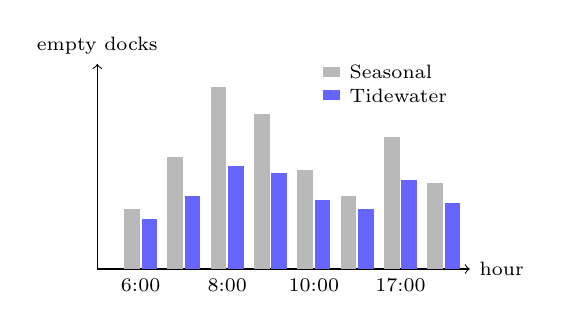
\begin{tikzpicture}[x=0.55cm,y=0.042cm]
    \draw[->] (0,0) -- (8.6,0) node[right] {\scriptsize hour};
    \draw[->] (0,0) -- (0,62) node[above] {\scriptsize empty docks};
    \foreach \h/\a/\b in {1/18/15,2/34/22,3/55/31,4/47/29,5/30/21,6/22/18,7/40/27,8/26/20}{
      \fill[gray!55] (\h-0.38,0) rectangle (\h-0.02,\a);
      \fill[blue!60] (\h+0.02,0) rectangle (\h+0.38,\b);
    }
    \foreach \h/\l in {1/6,3/8,5/10,7/17}{ \node[below] at (\h,0) {\scriptsize \l:00}; }
    \fill[gray!55] (5.2,58) rectangle (5.6,61); \node[right] at (5.6,59.5) {\scriptsize Seasonal};
    \fill[blue!60] (5.2,51) rectangle (5.6,54); \node[right] at (5.6,52.5) {\scriptsize Tidewater};
  \end{tikzpicture}
  \caption{Empty docks per hour on a rainy weekday. Tidewater anticipates the late morning peak and the evening event.}
  \label{fig:hourly}
\end{figure}

\paragraph{Rainy days and events.}
Figure~\ref{fig:hourly} follows a rainy weekday with a stadium event in the evening.
The seasonal baseline repeats the previous week and misses both the delayed morning peak and the evening surge.
Tidewater sees the rain in the context features and shifts the peak by about an hour.

\paragraph{New stations.}
When a station opens, Tidewater initialized from its neighbours reaches the accuracy of a fully trained head after five days, while the per-station model needs about a month.

\section{Conclusion}

Tidewater forecasts dock demand with a shared city-level encoder and small station heads.
It reduces empty-dock hours and truck distance on simulated networks and adapts quickly to new stations.
Future work will test the method on real trip records and couple it directly with a route planner.

\end{document}
